% ============================================================
% CSD 415 Project Phase I Final Review — Beamer slide deck
% Team: Shino (76), Stephin Arnold Raj S (66), Simranjeet Kour (56)
% Group 18, NSS College of Engineering | Guide: Reshma Sudhakaran
%
% HOW TO COMPILE
%   Normal deck (for presenting):
%       pdflatex final_review.tex
%       pdflatex final_review.tex   (run twice for TOC/refs to settle)
%
%   Handout for the guide's signature page (4 slides per page, no
%   animations/overlays). Either:
%     (a) pass the class option directly:
%         pdflatex "\PassOptionsToClass{handout}{beamer}% ============================================================
% CSD 415 Project Phase I Final Review — Beamer slide deck
% Team: Shino (76), Stephin Arnold Raj S (66), Simranjeet Kour (56)
% Group 18, NSS College of Engineering | Guide: Reshma Sudhakaran
%
% HOW TO COMPILE
%   Normal deck (for presenting):
%       pdflatex final_review.tex
%       pdflatex final_review.tex   (run twice for TOC/refs to settle)
%
%   Handout for the guide's signature page (4 slides per page, no
%   animations/overlays). Either:
%     (a) pass the class option directly:
%         pdflatex "\PassOptionsToClass{handout}{beamer}% ============================================================
% CSD 415 Project Phase I Final Review — Beamer slide deck
% Team: Shino (76), Stephin Arnold Raj S (66), Simranjeet Kour (56)
% Group 18, NSS College of Engineering | Guide: Reshma Sudhakaran
%
% HOW TO COMPILE
%   Normal deck (for presenting):
%       pdflatex final_review.tex
%       pdflatex final_review.tex   (run twice for TOC/refs to settle)
%
%   Handout for the guide's signature page (4 slides per page, no
%   animations/overlays). Either:
%     (a) pass the class option directly:
%         pdflatex "\PassOptionsToClass{handout}{beamer}% ============================================================
% CSD 415 Project Phase I Final Review — Beamer slide deck
% Team: Shino (76), Stephin Arnold Raj S (66), Simranjeet Kour (56)
% Group 18, NSS College of Engineering | Guide: Reshma Sudhakaran
%
% HOW TO COMPILE
%   Normal deck (for presenting):
%       pdflatex final_review.tex
%       pdflatex final_review.tex   (run twice for TOC/refs to settle)
%
%   Handout for the guide's signature page (4 slides per page, no
%   animations/overlays). Either:
%     (a) pass the class option directly:
%         pdflatex "\PassOptionsToClass{handout}{beamer}\input{final_review.tex}"
%     (b) or compile the companion file final_review_handout.tex
%         (same content, \documentclass[handout]{beamer} + pgfpages
%          4-up layout baked in) — see that file's header comment.
%
% HONESTY NOTE: every number on these slides must trace back to a file
% in this repo. Real pilot data was collected manually (300 queries via
% perplexity.ai, no paid API budget available) and real model metrics
% now exist in artifacts/metrics.json / data/pilot_stats.json — see
% docs/SLIDE_NUMBERS.md for the slide-by-slide source map.
% ============================================================

\documentclass[aspectratio=169]{beamer}

\usetheme{Madrid}
\usecolortheme{default}
\setbeamertemplate{navigation symbols}{}
\setbeamertemplate{footline}[frame number]

% ---- Custom navy / accent palette ----
\definecolor{navyPrimary}{RGB}{30,27,75}
\definecolor{navySecondary}{RGB}{49,46,129}
\definecolor{accentIndigo}{RGB}{67,56,202}
\definecolor{accentGreen}{RGB}{16,185,129}
\definecolor{accentRed}{RGB}{239,68,68}
\definecolor{lightBg}{RGB}{248,250,252}

\setbeamercolor{structure}{fg=navySecondary}
\setbeamercolor{palette primary}{bg=navyPrimary,fg=white}
\setbeamercolor{palette secondary}{bg=navySecondary,fg=white}
\setbeamercolor{palette tertiary}{bg=accentIndigo,fg=white}
\setbeamercolor{title}{fg=white}
\setbeamercolor{frametitle}{bg=navyPrimary,fg=white}
\setbeamercolor{background canvas}{bg=lightBg}
\setbeamercolor{block title}{bg=accentIndigo,fg=white}
\setbeamercolor{block body}{bg=white,fg=black}

% Larger body font, consistent with "~22pt" guidance
\setbeamerfont{frametitle}{size=\Large,series=\bfseries}
\setbeamerfont{normal text}{size=\large}
\setbeamerfont{itemize/enumerate body}{size=\large}

\usepackage[utf8]{inputenc}
\usepackage{tikz}
\usetikzlibrary{positioning,arrows.meta,shapes.geometric}
\usepackage{booktabs}
\usepackage{hyperref}

\title[Citation Likelihood Prediction]{Citation Likelihood Prediction\\in Generative Answer Engines}
\subtitle{Explainable ML Approach for Local Business Content}
\author{Shino (76) \quad Stephin Arnold Raj S (66) \quad Simranjeet Kour (56)}
\institute{CSD 415 Project Phase I\\Group 18, NSS College of Engineering\\Guide: Reshma Sudhakaran}
\date{22 October 2026}

\begin{document}

% ---------------- Title ----------------
\begin{frame}
  \titlepage
\end{frame}

% ---------------- Existing Methodology in detail ----------------
\begin{frame}{Existing Methodology (1/2): Post-hoc Trackers \& Checklists}
  \begin{itemize}
    \item \textbf{Post-hoc AI-visibility trackers} (e.g.\ the open-source Getcito/Elmo-style tool): periodically query answer engines and report \emph{whether} your page was cited.
    \begin{itemize}
      \item Tells you the outcome \emph{after} publication — no prediction before you write.
      \item No explanation of \emph{why} a page was or wasn't cited.
    \end{itemize}
    \item \textbf{Static rule / checklist auditors}: score a page against a fixed list (schema present? FAQ present? word count?).
    \begin{itemize}
      \item Transparent, but every rule has equal weight — no learning from outcomes.
      \item Cannot say \emph{how likely} citation is, only \emph{how many boxes are ticked}.
    \end{itemize}
  \end{itemize}
\end{frame}

\begin{frame}{Existing Methodology (2/2): Classical SEO Factor Studies}
  \begin{itemize}
    \item \textbf{Bataineh et al.\ (2025), \emph{Cogent Business \& Management}}: empirical PLS-SEM study — content quality, technical SEO, backlinks, and mobile-friendliness predict search \emph{rankings}, mediated by user engagement.
    \item Strong evidence for classical search ranking, but:
    \begin{itemize}
      \item Targets the 10-blue-links ranking problem, not AI-generated-answer citation.
      \item Correlational, structural-equation based — not a page-level, explainable, per-URL predictive model.
    \end{itemize}
    \item \textbf{Gap}: no existing tool learns a predictive, explainable model of \emph{citation} likelihood specifically for generative answer engines.
  \end{itemize}
\end{frame}

% ---------------- Need for Proposed Methodology ----------------
\begin{frame}{Need for Proposed Methodology}
  \begin{itemize}
    \item Generative answer engines (Perplexity, ChatGPT-style search) synthesize one answer and cite only \textbf{1--3} sources — very different from ranking 10 links.
    \item Businesses need to know \emph{before publishing} how citable a page is, and \emph{which} features to fix.
    \item Our approach: a \textbf{learned, explainable, pre-publication predictor} —
    \begin{itemize}
      \item XGBoost classifier trained on real citation outcomes (not a checklist).
      \item SHAP explains \emph{this classifier's} decision per page, per feature.
    \end{itemize}
    \item Positioned between post-hoc trackers (outcome only) and static checklists (no learning).
  \end{itemize}
\end{frame}

% ---------------- Datasets ----------------
\begin{frame}{Datasets}
  \begin{itemize}
    \item \textbf{Pilot design}: 200 real local-business search queries, 50 per category across 4 categories:
    \begin{itemize}
      \item Gyms (40 Indian cities) \quad\textbullet\quad Chauffeur/limo services (23 GCC cities)
      \item Kayaking/tour operators (35 Indian destinations) \quad\textbullet\quad Dental clinics (45 Indian cities)
    \end{itemize}
    \item \textbf{Label rule}: a page's canonical URL is labeled \texttt{1} if cited by Perplexity's \texttt{sonar} model for that query, else \texttt{0}. Candidate pool = cited URLs $\cup$ organic results.
    \item \textbf{Status — real data collected}: 300/300 queries collected (citations via \texttt{perplexity.ai}, tagged \texttt{collection\_method="manual\_web\_ui"} — no paid API budget was available); 978 unique candidate pages scraped, \textbf{592 usable rows} (189 cited / 403 not), \textbf{57.8\% scrape success rate}. Not flagged underpowered.
    \item Known limitation: negatives are drawn only from already-ranking pages, not a random web sample. 14\% of real citations went to directory/aggregator listings (JustDial, MagicPin, WhatClinic) rather than the business's own site.
  \end{itemize}
\end{frame}

% ---------------- Technology/Tools ----------------
\begin{frame}{Technology / Tools Specifications}
  \begin{columns}[T]
    \begin{column}{0.5\textwidth}
      \textbf{Collection \& Scraping}
      \begin{itemize}
        \item Python 3
        \item \texttt{requests}, \texttt{BeautifulSoup4}, \texttt{lxml}
        \item Perplexity API (\texttt{sonar}), SerpAPI (optional)
      \end{itemize}
      \textbf{App}
      \begin{itemize}
        \item Streamlit (interactive UI)
      \end{itemize}
    \end{column}
    \begin{column}{0.5\textwidth}
      \textbf{Modeling \& XAI}
      \begin{itemize}
        \item scikit-learn (baselines, GroupKFold)
        \item XGBoost (final classifier)
        \item SHAP (TreeExplainer)
      \end{itemize}
    \end{column}
  \end{columns}
  \vspace{0.3cm}
  \small\textit{Note: the repository also contains an unrelated open-source project (``Getcito'', forked from ``Elmo'', MIT licensed) that this project is layered on top of at the repo-root level only. That code is cited/attributed, not our work.}
\end{frame}

% ---------------- Data Collection / Partial Implementation ----------------
\begin{frame}{Data Collection / Partial Implementation}
  \begin{columns}[T]
    \begin{column}{0.48\textwidth}
      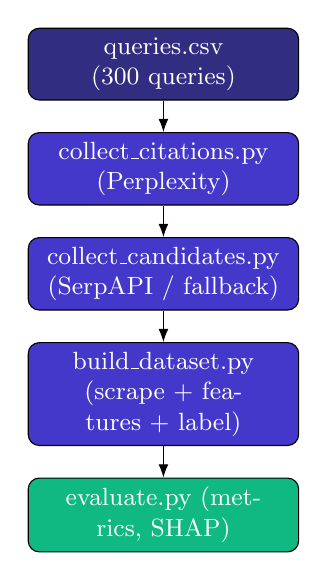
\begin{tikzpicture}[node distance=0.4cm, every node/.style={font=\small}]
        \node[draw, fill=navySecondary, text=white, rounded corners, text width=3.2cm, align=center] (q) {queries.csv (300 queries)};
        \node[draw, fill=accentIndigo, text=white, rounded corners, text width=3.2cm, align=center, below=of q] (cite) {collect\_citations.py (Perplexity)};
        \node[draw, fill=accentIndigo, text=white, rounded corners, text width=3.2cm, align=center, below=of cite] (cand) {collect\_candidates.py (SerpAPI / fallback)};
        \node[draw, fill=accentIndigo, text=white, rounded corners, text width=3.2cm, align=center, below=of cand] (build) {build\_dataset.py (scrape + features + label)};
        \node[draw, fill=accentGreen, text=white, rounded corners, text width=3.2cm, align=center, below=of build] (eval) {evaluate.py (metrics, SHAP)};
        \draw[-{Latex}] (q) -- (cite);
        \draw[-{Latex}] (cite) -- (cand);
        \draw[-{Latex}] (cand) -- (build);
        \draw[-{Latex}] (build) -- (eval);
      \end{tikzpicture}
    \end{column}
    \begin{column}{0.48\textwidth}
      \begin{itemize}
        \item All pipeline stages implemented and run end-to-end on real data.
        \item Cost-safety: \texttt{--dry-run}, \texttt{--max-calls} cap, on-disk caching, retry with backoff on every API call.
        \item Real pilot statistics: \textbf{300 queries, 592 usable rows, 57.8\% scrape success} (see \texttt{data/pilot\_stats.json}).
        \item \textit{[TODO (team): insert Streamlit app screenshot here]}
        \item \textit{[TODO (team): insert SHAP explanation screenshot here]}
      \end{itemize}
    \end{column}
  \end{columns}
\end{frame}

% ---------------- Results so far ----------------
\begin{frame}{Results So Far — Real Evaluation}
  \textbf{Evaluated on 592 real rows} (189 cited / 403 not), GroupKFold by domain ($k=5$, repeated 10$\times$ over shuffled row orders and pooled for a more precise estimate), all numbers from \texttt{artifacts/metrics.json}:
  \begin{itemize}
    \item \textbf{XGBoost}: ROC-AUC $0.69 \pm 0.06$, F1 $0.52 \pm 0.05$. \textbf{Logistic regression}: ROC-AUC $0.70 \pm 0.08$ — still numerically just ahead, but the gap has narrowed as the dataset grew (it was $0.69$ vs $0.64$ at the previous, smaller scale). Both clearly beat the rule-based checklist baseline (AUC $0.47$, at/below chance).
    \item \textbf{Label-shuffle sanity check}: AUC $0.56 \pm 0.05$ — close to chance, supporting \textbf{no major leakage}; the real signal is substantially genuine.
    \item \textbf{Feature-group ablation}: authority signals (schema, phone, address) are the strongest group (AUC $0.69$), ahead of structure ($0.66$) and content ($0.61$).
    \item \alert{Original repo's synthetic-trained model, evaluated on this real data: AUC $0.49$} — at chance, concretely confirming the circularity problem found in the Phase 1 audit (it claimed 88.8\% accuracy on its own synthetic labels).
    \item \textbf{SHAP stability} across folds: rank correlation $0.84$ — reasonably stable at this sample size.
  \end{itemize}
  \small Across three scales (100 $\to$ 200 $\to$ 300 queries), the AUC error bar has consistently tightened ($\pm0.19 \to \pm0.12 \to \pm0.06$) while the point estimate rose ($0.65 \to 0.64 \to 0.69$) — a real, honest trend, though accuracy at the default threshold has stayed near 63\% throughout, suggesting the remaining ceiling is more about label noise/feature richness than data volume alone. Full sanity checks, ablations, and SHAP figures in \texttt{artifacts/}.
\end{frame}

% ---------------- Conclusion & Future Work ----------------
\begin{frame}{Conclusion \& Future Work}
  \begin{itemize}
    \item Reframed GEO as a \textbf{learned, explainable, pre-publication prediction problem}, distinct from post-hoc trackers and static checklists.
    \item Built an honest, reproducible pipeline: query design $\to$ citation/candidate collection $\to$ labeled dataset $\to$ cross-validated evaluation $\to$ SHAP explanations.
    \item \textbf{Future work}:
    \begin{itemize}
      \item Scale to more queries, more cities, and multiple answer engines.
      \item Repeat queries (\texttt{--repeats}) to directly measure citation-label stability.
      \item Establish a retraining cadence as engine behavior drifts over time.
      \item Expand beyond local-business categories to test generality.
    \end{itemize}
  \end{itemize}
\end{frame}

% ---------------- Justification of Timeline ----------------
\begin{frame}{Justification of Timeline}
  \begin{columns}[T]
    \begin{column}{0.5\textwidth}
      \textbf{Semester 7 (delivered)}
      \begin{itemize}
        \item Codebase audit \& honesty fixes
        \item Real-data pilot: 300 queries collected (scaled up in three passes), 592-row dataset, full cross-validated evaluation \& SHAP analysis
        \item Ethics/cost-safety guardrails
        \item Documentation \& viva prep
      \end{itemize}
    \end{column}
    \begin{column}{0.5\textwidth}
      \textbf{Semester 8 (planned)}
      \begin{itemize}
        \item Scale to 300+ queries for narrower confidence intervals
        \item \texttt{--repeats} runs to measure citation-label stability
        \item App polish, offline demo snapshots
        \item Final report, diary, references
      \end{itemize}
    \end{column}
  \end{columns}
\end{frame}

% ---------------- References ----------------
\begin{frame}{References}
  \begin{itemize}
    \item Bataineh, A.\ et al.\ (2025). Empirical study of SEO ranking factors via PLS-SEM. \emph{Cogent Business \& Management}.
    \item Additional references: see \texttt{docs/REFERENCES\_TODO.md} — candidate journal references identified, impact-factor verification \textbf{TBD (team)} before the final report.
  \end{itemize}
\end{frame}

% ---------------- Thank you ----------------
\begin{frame}
  \centering
  {\Huge \color{navyPrimary} \textbf{Thank You}}\\[0.5cm]
  {\large Questions?}
\end{frame}

\end{document}
"
%     (b) or compile the companion file final_review_handout.tex
%         (same content, \documentclass[handout]{beamer} + pgfpages
%          4-up layout baked in) — see that file's header comment.
%
% HONESTY NOTE: every number on these slides must trace back to a file
% in this repo. Real pilot data was collected manually (300 queries via
% perplexity.ai, no paid API budget available) and real model metrics
% now exist in artifacts/metrics.json / data/pilot_stats.json — see
% docs/SLIDE_NUMBERS.md for the slide-by-slide source map.
% ============================================================

\documentclass[aspectratio=169]{beamer}

\usetheme{Madrid}
\usecolortheme{default}
\setbeamertemplate{navigation symbols}{}
\setbeamertemplate{footline}[frame number]

% ---- Custom navy / accent palette ----
\definecolor{navyPrimary}{RGB}{30,27,75}
\definecolor{navySecondary}{RGB}{49,46,129}
\definecolor{accentIndigo}{RGB}{67,56,202}
\definecolor{accentGreen}{RGB}{16,185,129}
\definecolor{accentRed}{RGB}{239,68,68}
\definecolor{lightBg}{RGB}{248,250,252}

\setbeamercolor{structure}{fg=navySecondary}
\setbeamercolor{palette primary}{bg=navyPrimary,fg=white}
\setbeamercolor{palette secondary}{bg=navySecondary,fg=white}
\setbeamercolor{palette tertiary}{bg=accentIndigo,fg=white}
\setbeamercolor{title}{fg=white}
\setbeamercolor{frametitle}{bg=navyPrimary,fg=white}
\setbeamercolor{background canvas}{bg=lightBg}
\setbeamercolor{block title}{bg=accentIndigo,fg=white}
\setbeamercolor{block body}{bg=white,fg=black}

% Larger body font, consistent with "~22pt" guidance
\setbeamerfont{frametitle}{size=\Large,series=\bfseries}
\setbeamerfont{normal text}{size=\large}
\setbeamerfont{itemize/enumerate body}{size=\large}

\usepackage[utf8]{inputenc}
\usepackage{tikz}
\usetikzlibrary{positioning,arrows.meta,shapes.geometric}
\usepackage{booktabs}
\usepackage{hyperref}

\title[Citation Likelihood Prediction]{Citation Likelihood Prediction\\in Generative Answer Engines}
\subtitle{Explainable ML Approach for Local Business Content}
\author{Shino (76) \quad Stephin Arnold Raj S (66) \quad Simranjeet Kour (56)}
\institute{CSD 415 Project Phase I\\Group 18, NSS College of Engineering\\Guide: Reshma Sudhakaran}
\date{22 October 2026}

\begin{document}

% ---------------- Title ----------------
\begin{frame}
  \titlepage
\end{frame}

% ---------------- Existing Methodology in detail ----------------
\begin{frame}{Existing Methodology (1/2): Post-hoc Trackers \& Checklists}
  \begin{itemize}
    \item \textbf{Post-hoc AI-visibility trackers} (e.g.\ the open-source Getcito/Elmo-style tool): periodically query answer engines and report \emph{whether} your page was cited.
    \begin{itemize}
      \item Tells you the outcome \emph{after} publication — no prediction before you write.
      \item No explanation of \emph{why} a page was or wasn't cited.
    \end{itemize}
    \item \textbf{Static rule / checklist auditors}: score a page against a fixed list (schema present? FAQ present? word count?).
    \begin{itemize}
      \item Transparent, but every rule has equal weight — no learning from outcomes.
      \item Cannot say \emph{how likely} citation is, only \emph{how many boxes are ticked}.
    \end{itemize}
  \end{itemize}
\end{frame}

\begin{frame}{Existing Methodology (2/2): Classical SEO Factor Studies}
  \begin{itemize}
    \item \textbf{Bataineh et al.\ (2025), \emph{Cogent Business \& Management}}: empirical PLS-SEM study — content quality, technical SEO, backlinks, and mobile-friendliness predict search \emph{rankings}, mediated by user engagement.
    \item Strong evidence for classical search ranking, but:
    \begin{itemize}
      \item Targets the 10-blue-links ranking problem, not AI-generated-answer citation.
      \item Correlational, structural-equation based — not a page-level, explainable, per-URL predictive model.
    \end{itemize}
    \item \textbf{Gap}: no existing tool learns a predictive, explainable model of \emph{citation} likelihood specifically for generative answer engines.
  \end{itemize}
\end{frame}

% ---------------- Need for Proposed Methodology ----------------
\begin{frame}{Need for Proposed Methodology}
  \begin{itemize}
    \item Generative answer engines (Perplexity, ChatGPT-style search) synthesize one answer and cite only \textbf{1--3} sources — very different from ranking 10 links.
    \item Businesses need to know \emph{before publishing} how citable a page is, and \emph{which} features to fix.
    \item Our approach: a \textbf{learned, explainable, pre-publication predictor} —
    \begin{itemize}
      \item XGBoost classifier trained on real citation outcomes (not a checklist).
      \item SHAP explains \emph{this classifier's} decision per page, per feature.
    \end{itemize}
    \item Positioned between post-hoc trackers (outcome only) and static checklists (no learning).
  \end{itemize}
\end{frame}

% ---------------- Datasets ----------------
\begin{frame}{Datasets}
  \begin{itemize}
    \item \textbf{Pilot design}: 200 real local-business search queries, 50 per category across 4 categories:
    \begin{itemize}
      \item Gyms (40 Indian cities) \quad\textbullet\quad Chauffeur/limo services (23 GCC cities)
      \item Kayaking/tour operators (35 Indian destinations) \quad\textbullet\quad Dental clinics (45 Indian cities)
    \end{itemize}
    \item \textbf{Label rule}: a page's canonical URL is labeled \texttt{1} if cited by Perplexity's \texttt{sonar} model for that query, else \texttt{0}. Candidate pool = cited URLs $\cup$ organic results.
    \item \textbf{Status — real data collected}: 300/300 queries collected (citations via \texttt{perplexity.ai}, tagged \texttt{collection\_method="manual\_web\_ui"} — no paid API budget was available); 978 unique candidate pages scraped, \textbf{592 usable rows} (189 cited / 403 not), \textbf{57.8\% scrape success rate}. Not flagged underpowered.
    \item Known limitation: negatives are drawn only from already-ranking pages, not a random web sample. 14\% of real citations went to directory/aggregator listings (JustDial, MagicPin, WhatClinic) rather than the business's own site.
  \end{itemize}
\end{frame}

% ---------------- Technology/Tools ----------------
\begin{frame}{Technology / Tools Specifications}
  \begin{columns}[T]
    \begin{column}{0.5\textwidth}
      \textbf{Collection \& Scraping}
      \begin{itemize}
        \item Python 3
        \item \texttt{requests}, \texttt{BeautifulSoup4}, \texttt{lxml}
        \item Perplexity API (\texttt{sonar}), SerpAPI (optional)
      \end{itemize}
      \textbf{App}
      \begin{itemize}
        \item Streamlit (interactive UI)
      \end{itemize}
    \end{column}
    \begin{column}{0.5\textwidth}
      \textbf{Modeling \& XAI}
      \begin{itemize}
        \item scikit-learn (baselines, GroupKFold)
        \item XGBoost (final classifier)
        \item SHAP (TreeExplainer)
      \end{itemize}
    \end{column}
  \end{columns}
  \vspace{0.3cm}
  \small\textit{Note: the repository also contains an unrelated open-source project (``Getcito'', forked from ``Elmo'', MIT licensed) that this project is layered on top of at the repo-root level only. That code is cited/attributed, not our work.}
\end{frame}

% ---------------- Data Collection / Partial Implementation ----------------
\begin{frame}{Data Collection / Partial Implementation}
  \begin{columns}[T]
    \begin{column}{0.48\textwidth}
      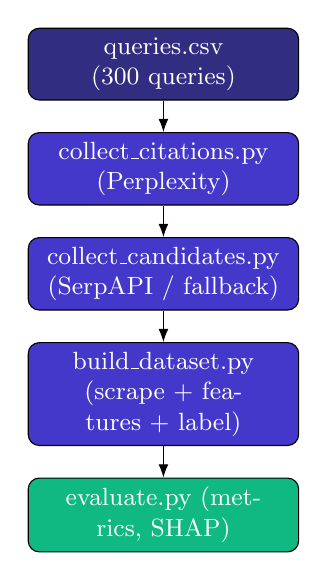
\begin{tikzpicture}[node distance=0.4cm, every node/.style={font=\small}]
        \node[draw, fill=navySecondary, text=white, rounded corners, text width=3.2cm, align=center] (q) {queries.csv (300 queries)};
        \node[draw, fill=accentIndigo, text=white, rounded corners, text width=3.2cm, align=center, below=of q] (cite) {collect\_citations.py (Perplexity)};
        \node[draw, fill=accentIndigo, text=white, rounded corners, text width=3.2cm, align=center, below=of cite] (cand) {collect\_candidates.py (SerpAPI / fallback)};
        \node[draw, fill=accentIndigo, text=white, rounded corners, text width=3.2cm, align=center, below=of cand] (build) {build\_dataset.py (scrape + features + label)};
        \node[draw, fill=accentGreen, text=white, rounded corners, text width=3.2cm, align=center, below=of build] (eval) {evaluate.py (metrics, SHAP)};
        \draw[-{Latex}] (q) -- (cite);
        \draw[-{Latex}] (cite) -- (cand);
        \draw[-{Latex}] (cand) -- (build);
        \draw[-{Latex}] (build) -- (eval);
      \end{tikzpicture}
    \end{column}
    \begin{column}{0.48\textwidth}
      \begin{itemize}
        \item All pipeline stages implemented and run end-to-end on real data.
        \item Cost-safety: \texttt{--dry-run}, \texttt{--max-calls} cap, on-disk caching, retry with backoff on every API call.
        \item Real pilot statistics: \textbf{300 queries, 592 usable rows, 57.8\% scrape success} (see \texttt{data/pilot\_stats.json}).
        \item \textit{[TODO (team): insert Streamlit app screenshot here]}
        \item \textit{[TODO (team): insert SHAP explanation screenshot here]}
      \end{itemize}
    \end{column}
  \end{columns}
\end{frame}

% ---------------- Results so far ----------------
\begin{frame}{Results So Far — Real Evaluation}
  \textbf{Evaluated on 592 real rows} (189 cited / 403 not), GroupKFold by domain ($k=5$, repeated 10$\times$ over shuffled row orders and pooled for a more precise estimate), all numbers from \texttt{artifacts/metrics.json}:
  \begin{itemize}
    \item \textbf{XGBoost}: ROC-AUC $0.69 \pm 0.06$, F1 $0.52 \pm 0.05$. \textbf{Logistic regression}: ROC-AUC $0.70 \pm 0.08$ — still numerically just ahead, but the gap has narrowed as the dataset grew (it was $0.69$ vs $0.64$ at the previous, smaller scale). Both clearly beat the rule-based checklist baseline (AUC $0.47$, at/below chance).
    \item \textbf{Label-shuffle sanity check}: AUC $0.56 \pm 0.05$ — close to chance, supporting \textbf{no major leakage}; the real signal is substantially genuine.
    \item \textbf{Feature-group ablation}: authority signals (schema, phone, address) are the strongest group (AUC $0.69$), ahead of structure ($0.66$) and content ($0.61$).
    \item \alert{Original repo's synthetic-trained model, evaluated on this real data: AUC $0.49$} — at chance, concretely confirming the circularity problem found in the Phase 1 audit (it claimed 88.8\% accuracy on its own synthetic labels).
    \item \textbf{SHAP stability} across folds: rank correlation $0.84$ — reasonably stable at this sample size.
  \end{itemize}
  \small Across three scales (100 $\to$ 200 $\to$ 300 queries), the AUC error bar has consistently tightened ($\pm0.19 \to \pm0.12 \to \pm0.06$) while the point estimate rose ($0.65 \to 0.64 \to 0.69$) — a real, honest trend, though accuracy at the default threshold has stayed near 63\% throughout, suggesting the remaining ceiling is more about label noise/feature richness than data volume alone. Full sanity checks, ablations, and SHAP figures in \texttt{artifacts/}.
\end{frame}

% ---------------- Conclusion & Future Work ----------------
\begin{frame}{Conclusion \& Future Work}
  \begin{itemize}
    \item Reframed GEO as a \textbf{learned, explainable, pre-publication prediction problem}, distinct from post-hoc trackers and static checklists.
    \item Built an honest, reproducible pipeline: query design $\to$ citation/candidate collection $\to$ labeled dataset $\to$ cross-validated evaluation $\to$ SHAP explanations.
    \item \textbf{Future work}:
    \begin{itemize}
      \item Scale to more queries, more cities, and multiple answer engines.
      \item Repeat queries (\texttt{--repeats}) to directly measure citation-label stability.
      \item Establish a retraining cadence as engine behavior drifts over time.
      \item Expand beyond local-business categories to test generality.
    \end{itemize}
  \end{itemize}
\end{frame}

% ---------------- Justification of Timeline ----------------
\begin{frame}{Justification of Timeline}
  \begin{columns}[T]
    \begin{column}{0.5\textwidth}
      \textbf{Semester 7 (delivered)}
      \begin{itemize}
        \item Codebase audit \& honesty fixes
        \item Real-data pilot: 300 queries collected (scaled up in three passes), 592-row dataset, full cross-validated evaluation \& SHAP analysis
        \item Ethics/cost-safety guardrails
        \item Documentation \& viva prep
      \end{itemize}
    \end{column}
    \begin{column}{0.5\textwidth}
      \textbf{Semester 8 (planned)}
      \begin{itemize}
        \item Scale to 300+ queries for narrower confidence intervals
        \item \texttt{--repeats} runs to measure citation-label stability
        \item App polish, offline demo snapshots
        \item Final report, diary, references
      \end{itemize}
    \end{column}
  \end{columns}
\end{frame}

% ---------------- References ----------------
\begin{frame}{References}
  \begin{itemize}
    \item Bataineh, A.\ et al.\ (2025). Empirical study of SEO ranking factors via PLS-SEM. \emph{Cogent Business \& Management}.
    \item Additional references: see \texttt{docs/REFERENCES\_TODO.md} — candidate journal references identified, impact-factor verification \textbf{TBD (team)} before the final report.
  \end{itemize}
\end{frame}

% ---------------- Thank you ----------------
\begin{frame}
  \centering
  {\Huge \color{navyPrimary} \textbf{Thank You}}\\[0.5cm]
  {\large Questions?}
\end{frame}

\end{document}
"
%     (b) or compile the companion file final_review_handout.tex
%         (same content, \documentclass[handout]{beamer} + pgfpages
%          4-up layout baked in) — see that file's header comment.
%
% HONESTY NOTE: every number on these slides must trace back to a file
% in this repo. Real pilot data was collected manually (300 queries via
% perplexity.ai, no paid API budget available) and real model metrics
% now exist in artifacts/metrics.json / data/pilot_stats.json — see
% docs/SLIDE_NUMBERS.md for the slide-by-slide source map.
% ============================================================

\documentclass[aspectratio=169]{beamer}

\usetheme{Madrid}
\usecolortheme{default}
\setbeamertemplate{navigation symbols}{}
\setbeamertemplate{footline}[frame number]

% ---- Custom navy / accent palette ----
\definecolor{navyPrimary}{RGB}{30,27,75}
\definecolor{navySecondary}{RGB}{49,46,129}
\definecolor{accentIndigo}{RGB}{67,56,202}
\definecolor{accentGreen}{RGB}{16,185,129}
\definecolor{accentRed}{RGB}{239,68,68}
\definecolor{lightBg}{RGB}{248,250,252}

\setbeamercolor{structure}{fg=navySecondary}
\setbeamercolor{palette primary}{bg=navyPrimary,fg=white}
\setbeamercolor{palette secondary}{bg=navySecondary,fg=white}
\setbeamercolor{palette tertiary}{bg=accentIndigo,fg=white}
\setbeamercolor{title}{fg=white}
\setbeamercolor{frametitle}{bg=navyPrimary,fg=white}
\setbeamercolor{background canvas}{bg=lightBg}
\setbeamercolor{block title}{bg=accentIndigo,fg=white}
\setbeamercolor{block body}{bg=white,fg=black}

% Larger body font, consistent with "~22pt" guidance
\setbeamerfont{frametitle}{size=\Large,series=\bfseries}
\setbeamerfont{normal text}{size=\large}
\setbeamerfont{itemize/enumerate body}{size=\large}

\usepackage[utf8]{inputenc}
\usepackage{tikz}
\usetikzlibrary{positioning,arrows.meta,shapes.geometric}
\usepackage{booktabs}
\usepackage{hyperref}

\title[Citation Likelihood Prediction]{Citation Likelihood Prediction\\in Generative Answer Engines}
\subtitle{Explainable ML Approach for Local Business Content}
\author{Shino (76) \quad Stephin Arnold Raj S (66) \quad Simranjeet Kour (56)}
\institute{CSD 415 Project Phase I\\Group 18, NSS College of Engineering\\Guide: Reshma Sudhakaran}
\date{22 October 2026}

\begin{document}

% ---------------- Title ----------------
\begin{frame}
  \titlepage
\end{frame}

% ---------------- Existing Methodology in detail ----------------
\begin{frame}{Existing Methodology (1/2): Post-hoc Trackers \& Checklists}
  \begin{itemize}
    \item \textbf{Post-hoc AI-visibility trackers} (e.g.\ the open-source Getcito/Elmo-style tool): periodically query answer engines and report \emph{whether} your page was cited.
    \begin{itemize}
      \item Tells you the outcome \emph{after} publication — no prediction before you write.
      \item No explanation of \emph{why} a page was or wasn't cited.
    \end{itemize}
    \item \textbf{Static rule / checklist auditors}: score a page against a fixed list (schema present? FAQ present? word count?).
    \begin{itemize}
      \item Transparent, but every rule has equal weight — no learning from outcomes.
      \item Cannot say \emph{how likely} citation is, only \emph{how many boxes are ticked}.
    \end{itemize}
  \end{itemize}
\end{frame}

\begin{frame}{Existing Methodology (2/2): Classical SEO Factor Studies}
  \begin{itemize}
    \item \textbf{Bataineh et al.\ (2025), \emph{Cogent Business \& Management}}: empirical PLS-SEM study — content quality, technical SEO, backlinks, and mobile-friendliness predict search \emph{rankings}, mediated by user engagement.
    \item Strong evidence for classical search ranking, but:
    \begin{itemize}
      \item Targets the 10-blue-links ranking problem, not AI-generated-answer citation.
      \item Correlational, structural-equation based — not a page-level, explainable, per-URL predictive model.
    \end{itemize}
    \item \textbf{Gap}: no existing tool learns a predictive, explainable model of \emph{citation} likelihood specifically for generative answer engines.
  \end{itemize}
\end{frame}

% ---------------- Need for Proposed Methodology ----------------
\begin{frame}{Need for Proposed Methodology}
  \begin{itemize}
    \item Generative answer engines (Perplexity, ChatGPT-style search) synthesize one answer and cite only \textbf{1--3} sources — very different from ranking 10 links.
    \item Businesses need to know \emph{before publishing} how citable a page is, and \emph{which} features to fix.
    \item Our approach: a \textbf{learned, explainable, pre-publication predictor} —
    \begin{itemize}
      \item XGBoost classifier trained on real citation outcomes (not a checklist).
      \item SHAP explains \emph{this classifier's} decision per page, per feature.
    \end{itemize}
    \item Positioned between post-hoc trackers (outcome only) and static checklists (no learning).
  \end{itemize}
\end{frame}

% ---------------- Datasets ----------------
\begin{frame}{Datasets}
  \begin{itemize}
    \item \textbf{Pilot design}: 200 real local-business search queries, 50 per category across 4 categories:
    \begin{itemize}
      \item Gyms (40 Indian cities) \quad\textbullet\quad Chauffeur/limo services (23 GCC cities)
      \item Kayaking/tour operators (35 Indian destinations) \quad\textbullet\quad Dental clinics (45 Indian cities)
    \end{itemize}
    \item \textbf{Label rule}: a page's canonical URL is labeled \texttt{1} if cited by Perplexity's \texttt{sonar} model for that query, else \texttt{0}. Candidate pool = cited URLs $\cup$ organic results.
    \item \textbf{Status — real data collected}: 300/300 queries collected (citations via \texttt{perplexity.ai}, tagged \texttt{collection\_method="manual\_web\_ui"} — no paid API budget was available); 978 unique candidate pages scraped, \textbf{592 usable rows} (189 cited / 403 not), \textbf{57.8\% scrape success rate}. Not flagged underpowered.
    \item Known limitation: negatives are drawn only from already-ranking pages, not a random web sample. 14\% of real citations went to directory/aggregator listings (JustDial, MagicPin, WhatClinic) rather than the business's own site.
  \end{itemize}
\end{frame}

% ---------------- Technology/Tools ----------------
\begin{frame}{Technology / Tools Specifications}
  \begin{columns}[T]
    \begin{column}{0.5\textwidth}
      \textbf{Collection \& Scraping}
      \begin{itemize}
        \item Python 3
        \item \texttt{requests}, \texttt{BeautifulSoup4}, \texttt{lxml}
        \item Perplexity API (\texttt{sonar}), SerpAPI (optional)
      \end{itemize}
      \textbf{App}
      \begin{itemize}
        \item Streamlit (interactive UI)
      \end{itemize}
    \end{column}
    \begin{column}{0.5\textwidth}
      \textbf{Modeling \& XAI}
      \begin{itemize}
        \item scikit-learn (baselines, GroupKFold)
        \item XGBoost (final classifier)
        \item SHAP (TreeExplainer)
      \end{itemize}
    \end{column}
  \end{columns}
  \vspace{0.3cm}
  \small\textit{Note: the repository also contains an unrelated open-source project (``Getcito'', forked from ``Elmo'', MIT licensed) that this project is layered on top of at the repo-root level only. That code is cited/attributed, not our work.}
\end{frame}

% ---------------- Data Collection / Partial Implementation ----------------
\begin{frame}{Data Collection / Partial Implementation}
  \begin{columns}[T]
    \begin{column}{0.48\textwidth}
      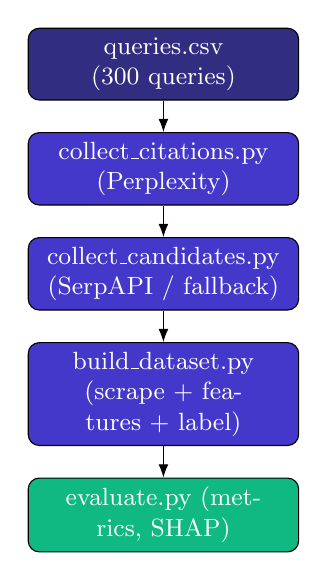
\begin{tikzpicture}[node distance=0.4cm, every node/.style={font=\small}]
        \node[draw, fill=navySecondary, text=white, rounded corners, text width=3.2cm, align=center] (q) {queries.csv (300 queries)};
        \node[draw, fill=accentIndigo, text=white, rounded corners, text width=3.2cm, align=center, below=of q] (cite) {collect\_citations.py (Perplexity)};
        \node[draw, fill=accentIndigo, text=white, rounded corners, text width=3.2cm, align=center, below=of cite] (cand) {collect\_candidates.py (SerpAPI / fallback)};
        \node[draw, fill=accentIndigo, text=white, rounded corners, text width=3.2cm, align=center, below=of cand] (build) {build\_dataset.py (scrape + features + label)};
        \node[draw, fill=accentGreen, text=white, rounded corners, text width=3.2cm, align=center, below=of build] (eval) {evaluate.py (metrics, SHAP)};
        \draw[-{Latex}] (q) -- (cite);
        \draw[-{Latex}] (cite) -- (cand);
        \draw[-{Latex}] (cand) -- (build);
        \draw[-{Latex}] (build) -- (eval);
      \end{tikzpicture}
    \end{column}
    \begin{column}{0.48\textwidth}
      \begin{itemize}
        \item All pipeline stages implemented and run end-to-end on real data.
        \item Cost-safety: \texttt{--dry-run}, \texttt{--max-calls} cap, on-disk caching, retry with backoff on every API call.
        \item Real pilot statistics: \textbf{300 queries, 592 usable rows, 57.8\% scrape success} (see \texttt{data/pilot\_stats.json}).
        \item \textit{[TODO (team): insert Streamlit app screenshot here]}
        \item \textit{[TODO (team): insert SHAP explanation screenshot here]}
      \end{itemize}
    \end{column}
  \end{columns}
\end{frame}

% ---------------- Results so far ----------------
\begin{frame}{Results So Far — Real Evaluation}
  \textbf{Evaluated on 592 real rows} (189 cited / 403 not), GroupKFold by domain ($k=5$, repeated 10$\times$ over shuffled row orders and pooled for a more precise estimate), all numbers from \texttt{artifacts/metrics.json}:
  \begin{itemize}
    \item \textbf{XGBoost}: ROC-AUC $0.69 \pm 0.06$, F1 $0.52 \pm 0.05$. \textbf{Logistic regression}: ROC-AUC $0.70 \pm 0.08$ — still numerically just ahead, but the gap has narrowed as the dataset grew (it was $0.69$ vs $0.64$ at the previous, smaller scale). Both clearly beat the rule-based checklist baseline (AUC $0.47$, at/below chance).
    \item \textbf{Label-shuffle sanity check}: AUC $0.56 \pm 0.05$ — close to chance, supporting \textbf{no major leakage}; the real signal is substantially genuine.
    \item \textbf{Feature-group ablation}: authority signals (schema, phone, address) are the strongest group (AUC $0.69$), ahead of structure ($0.66$) and content ($0.61$).
    \item \alert{Original repo's synthetic-trained model, evaluated on this real data: AUC $0.49$} — at chance, concretely confirming the circularity problem found in the Phase 1 audit (it claimed 88.8\% accuracy on its own synthetic labels).
    \item \textbf{SHAP stability} across folds: rank correlation $0.84$ — reasonably stable at this sample size.
  \end{itemize}
  \small Across three scales (100 $\to$ 200 $\to$ 300 queries), the AUC error bar has consistently tightened ($\pm0.19 \to \pm0.12 \to \pm0.06$) while the point estimate rose ($0.65 \to 0.64 \to 0.69$) — a real, honest trend, though accuracy at the default threshold has stayed near 63\% throughout, suggesting the remaining ceiling is more about label noise/feature richness than data volume alone. Full sanity checks, ablations, and SHAP figures in \texttt{artifacts/}.
\end{frame}

% ---------------- Conclusion & Future Work ----------------
\begin{frame}{Conclusion \& Future Work}
  \begin{itemize}
    \item Reframed GEO as a \textbf{learned, explainable, pre-publication prediction problem}, distinct from post-hoc trackers and static checklists.
    \item Built an honest, reproducible pipeline: query design $\to$ citation/candidate collection $\to$ labeled dataset $\to$ cross-validated evaluation $\to$ SHAP explanations.
    \item \textbf{Future work}:
    \begin{itemize}
      \item Scale to more queries, more cities, and multiple answer engines.
      \item Repeat queries (\texttt{--repeats}) to directly measure citation-label stability.
      \item Establish a retraining cadence as engine behavior drifts over time.
      \item Expand beyond local-business categories to test generality.
    \end{itemize}
  \end{itemize}
\end{frame}

% ---------------- Justification of Timeline ----------------
\begin{frame}{Justification of Timeline}
  \begin{columns}[T]
    \begin{column}{0.5\textwidth}
      \textbf{Semester 7 (delivered)}
      \begin{itemize}
        \item Codebase audit \& honesty fixes
        \item Real-data pilot: 300 queries collected (scaled up in three passes), 592-row dataset, full cross-validated evaluation \& SHAP analysis
        \item Ethics/cost-safety guardrails
        \item Documentation \& viva prep
      \end{itemize}
    \end{column}
    \begin{column}{0.5\textwidth}
      \textbf{Semester 8 (planned)}
      \begin{itemize}
        \item Scale to 300+ queries for narrower confidence intervals
        \item \texttt{--repeats} runs to measure citation-label stability
        \item App polish, offline demo snapshots
        \item Final report, diary, references
      \end{itemize}
    \end{column}
  \end{columns}
\end{frame}

% ---------------- References ----------------
\begin{frame}{References}
  \begin{itemize}
    \item Bataineh, A.\ et al.\ (2025). Empirical study of SEO ranking factors via PLS-SEM. \emph{Cogent Business \& Management}.
    \item Additional references: see \texttt{docs/REFERENCES\_TODO.md} — candidate journal references identified, impact-factor verification \textbf{TBD (team)} before the final report.
  \end{itemize}
\end{frame}

% ---------------- Thank you ----------------
\begin{frame}
  \centering
  {\Huge \color{navyPrimary} \textbf{Thank You}}\\[0.5cm]
  {\large Questions?}
\end{frame}

\end{document}
"
%     (b) or compile the companion file final_review_handout.tex
%         (same content, \documentclass[handout]{beamer} + pgfpages
%          4-up layout baked in) — see that file's header comment.
%
% HONESTY NOTE: every number on these slides must trace back to a file
% in this repo. Real pilot data was collected manually (300 queries via
% perplexity.ai, no paid API budget available) and real model metrics
% now exist in artifacts/metrics.json / data/pilot_stats.json — see
% docs/SLIDE_NUMBERS.md for the slide-by-slide source map.
% ============================================================

\documentclass[aspectratio=169]{beamer}

\usetheme{Madrid}
\usecolortheme{default}
\setbeamertemplate{navigation symbols}{}
\setbeamertemplate{footline}[frame number]

% ---- Custom navy / accent palette ----
\definecolor{navyPrimary}{RGB}{30,27,75}
\definecolor{navySecondary}{RGB}{49,46,129}
\definecolor{accentIndigo}{RGB}{67,56,202}
\definecolor{accentGreen}{RGB}{16,185,129}
\definecolor{accentRed}{RGB}{239,68,68}
\definecolor{lightBg}{RGB}{248,250,252}

\setbeamercolor{structure}{fg=navySecondary}
\setbeamercolor{palette primary}{bg=navyPrimary,fg=white}
\setbeamercolor{palette secondary}{bg=navySecondary,fg=white}
\setbeamercolor{palette tertiary}{bg=accentIndigo,fg=white}
\setbeamercolor{title}{fg=white}
\setbeamercolor{frametitle}{bg=navyPrimary,fg=white}
\setbeamercolor{background canvas}{bg=lightBg}
\setbeamercolor{block title}{bg=accentIndigo,fg=white}
\setbeamercolor{block body}{bg=white,fg=black}

% Larger body font, consistent with "~22pt" guidance
\setbeamerfont{frametitle}{size=\Large,series=\bfseries}
\setbeamerfont{normal text}{size=\large}
\setbeamerfont{itemize/enumerate body}{size=\large}

\usepackage[utf8]{inputenc}
\usepackage{tikz}
\usetikzlibrary{positioning,arrows.meta,shapes.geometric}
\usepackage{booktabs}
\usepackage{hyperref}

\title[Citation Likelihood Prediction]{Citation Likelihood Prediction\\in Generative Answer Engines}
\subtitle{Explainable ML Approach for Local Business Content}
\author{Shino (76) \quad Stephin Arnold Raj S (66) \quad Simranjeet Kour (56)}
\institute{CSD 415 Project Phase I\\Group 18, NSS College of Engineering\\Guide: Reshma Sudhakaran}
\date{22 October 2026}

\begin{document}

% ---------------- Title ----------------
\begin{frame}
  \titlepage
\end{frame}

% ---------------- Existing Methodology in detail ----------------
\begin{frame}{Existing Methodology (1/2): Post-hoc Trackers \& Checklists}
  \begin{itemize}
    \item \textbf{Post-hoc AI-visibility trackers} (e.g.\ the open-source Getcito/Elmo-style tool): periodically query answer engines and report \emph{whether} your page was cited.
    \begin{itemize}
      \item Tells you the outcome \emph{after} publication — no prediction before you write.
      \item No explanation of \emph{why} a page was or wasn't cited.
    \end{itemize}
    \item \textbf{Static rule / checklist auditors}: score a page against a fixed list (schema present? FAQ present? word count?).
    \begin{itemize}
      \item Transparent, but every rule has equal weight — no learning from outcomes.
      \item Cannot say \emph{how likely} citation is, only \emph{how many boxes are ticked}.
    \end{itemize}
  \end{itemize}
\end{frame}

\begin{frame}{Existing Methodology (2/2): Classical SEO Factor Studies}
  \begin{itemize}
    \item \textbf{Bataineh et al.\ (2025), \emph{Cogent Business \& Management}}: empirical PLS-SEM study — content quality, technical SEO, backlinks, and mobile-friendliness predict search \emph{rankings}, mediated by user engagement.
    \item Strong evidence for classical search ranking, but:
    \begin{itemize}
      \item Targets the 10-blue-links ranking problem, not AI-generated-answer citation.
      \item Correlational, structural-equation based — not a page-level, explainable, per-URL predictive model.
    \end{itemize}
    \item \textbf{Gap}: no existing tool learns a predictive, explainable model of \emph{citation} likelihood specifically for generative answer engines.
  \end{itemize}
\end{frame}

% ---------------- Need for Proposed Methodology ----------------
\begin{frame}{Need for Proposed Methodology}
  \begin{itemize}
    \item Generative answer engines (Perplexity, ChatGPT-style search) synthesize one answer and cite only \textbf{1--3} sources — very different from ranking 10 links.
    \item Businesses need to know \emph{before publishing} how citable a page is, and \emph{which} features to fix.
    \item Our approach: a \textbf{learned, explainable, pre-publication predictor} —
    \begin{itemize}
      \item XGBoost classifier trained on real citation outcomes (not a checklist).
      \item SHAP explains \emph{this classifier's} decision per page, per feature.
    \end{itemize}
    \item Positioned between post-hoc trackers (outcome only) and static checklists (no learning).
  \end{itemize}
\end{frame}

% ---------------- Datasets ----------------
\begin{frame}{Datasets}
  \begin{itemize}
    \item \textbf{Pilot design}: 200 real local-business search queries, 50 per category across 4 categories:
    \begin{itemize}
      \item Gyms (40 Indian cities) \quad\textbullet\quad Chauffeur/limo services (23 GCC cities)
      \item Kayaking/tour operators (35 Indian destinations) \quad\textbullet\quad Dental clinics (45 Indian cities)
    \end{itemize}
    \item \textbf{Label rule}: a page's canonical URL is labeled \texttt{1} if cited by Perplexity's \texttt{sonar} model for that query, else \texttt{0}. Candidate pool = cited URLs $\cup$ organic results.
    \item \textbf{Status — real data collected}: 300/300 queries collected (citations via \texttt{perplexity.ai}, tagged \texttt{collection\_method="manual\_web\_ui"} — no paid API budget was available); 978 unique candidate pages scraped, \textbf{592 usable rows} (189 cited / 403 not), \textbf{57.8\% scrape success rate}. Not flagged underpowered.
    \item Known limitation: negatives are drawn only from already-ranking pages, not a random web sample. 14\% of real citations went to directory/aggregator listings (JustDial, MagicPin, WhatClinic) rather than the business's own site.
  \end{itemize}
\end{frame}

% ---------------- Technology/Tools ----------------
\begin{frame}{Technology / Tools Specifications}
  \begin{columns}[T]
    \begin{column}{0.5\textwidth}
      \textbf{Collection \& Scraping}
      \begin{itemize}
        \item Python 3
        \item \texttt{requests}, \texttt{BeautifulSoup4}, \texttt{lxml}
        \item Perplexity API (\texttt{sonar}), SerpAPI (optional)
      \end{itemize}
      \textbf{App}
      \begin{itemize}
        \item Streamlit (interactive UI)
      \end{itemize}
    \end{column}
    \begin{column}{0.5\textwidth}
      \textbf{Modeling \& XAI}
      \begin{itemize}
        \item scikit-learn (baselines, GroupKFold)
        \item XGBoost (final classifier)
        \item SHAP (TreeExplainer)
      \end{itemize}
    \end{column}
  \end{columns}
  \vspace{0.3cm}
  \small\textit{Note: the repository also contains an unrelated open-source project (``Getcito'', forked from ``Elmo'', MIT licensed) that this project is layered on top of at the repo-root level only. That code is cited/attributed, not our work.}
\end{frame}

% ---------------- Data Collection / Partial Implementation ----------------
\begin{frame}{Data Collection / Partial Implementation}
  \begin{columns}[T]
    \begin{column}{0.48\textwidth}
      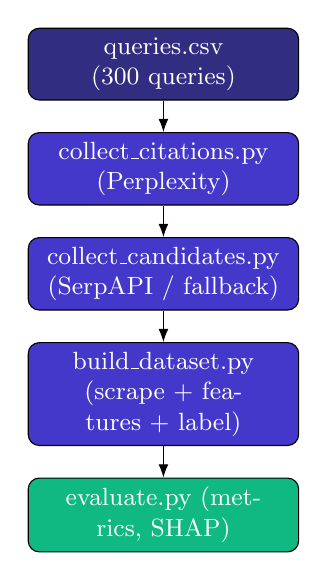
\begin{tikzpicture}[node distance=0.4cm, every node/.style={font=\small}]
        \node[draw, fill=navySecondary, text=white, rounded corners, text width=3.2cm, align=center] (q) {queries.csv (300 queries)};
        \node[draw, fill=accentIndigo, text=white, rounded corners, text width=3.2cm, align=center, below=of q] (cite) {collect\_citations.py (Perplexity)};
        \node[draw, fill=accentIndigo, text=white, rounded corners, text width=3.2cm, align=center, below=of cite] (cand) {collect\_candidates.py (SerpAPI / fallback)};
        \node[draw, fill=accentIndigo, text=white, rounded corners, text width=3.2cm, align=center, below=of cand] (build) {build\_dataset.py (scrape + features + label)};
        \node[draw, fill=accentGreen, text=white, rounded corners, text width=3.2cm, align=center, below=of build] (eval) {evaluate.py (metrics, SHAP)};
        \draw[-{Latex}] (q) -- (cite);
        \draw[-{Latex}] (cite) -- (cand);
        \draw[-{Latex}] (cand) -- (build);
        \draw[-{Latex}] (build) -- (eval);
      \end{tikzpicture}
    \end{column}
    \begin{column}{0.48\textwidth}
      \begin{itemize}
        \item All pipeline stages implemented and run end-to-end on real data.
        \item Cost-safety: \texttt{--dry-run}, \texttt{--max-calls} cap, on-disk caching, retry with backoff on every API call.
        \item Real pilot statistics: \textbf{300 queries, 592 usable rows, 57.8\% scrape success} (see \texttt{data/pilot\_stats.json}).
        \item \textit{[TODO (team): insert Streamlit app screenshot here]}
        \item \textit{[TODO (team): insert SHAP explanation screenshot here]}
      \end{itemize}
    \end{column}
  \end{columns}
\end{frame}

% ---------------- Results so far ----------------
\begin{frame}{Results So Far — Real Evaluation}
  \textbf{Evaluated on 592 real rows} (189 cited / 403 not), GroupKFold by domain ($k=5$, repeated 10$\times$ over shuffled row orders and pooled for a more precise estimate), all numbers from \texttt{artifacts/metrics.json}:
  \begin{itemize}
    \item \textbf{XGBoost}: ROC-AUC $0.69 \pm 0.06$, F1 $0.52 \pm 0.05$. \textbf{Logistic regression}: ROC-AUC $0.70 \pm 0.08$ — still numerically just ahead, but the gap has narrowed as the dataset grew (it was $0.69$ vs $0.64$ at the previous, smaller scale). Both clearly beat the rule-based checklist baseline (AUC $0.47$, at/below chance).
    \item \textbf{Label-shuffle sanity check}: AUC $0.56 \pm 0.05$ — close to chance, supporting \textbf{no major leakage}; the real signal is substantially genuine.
    \item \textbf{Feature-group ablation}: authority signals (schema, phone, address) are the strongest group (AUC $0.69$), ahead of structure ($0.66$) and content ($0.61$).
    \item \alert{Original repo's synthetic-trained model, evaluated on this real data: AUC $0.49$} — at chance, concretely confirming the circularity problem found in the Phase 1 audit (it claimed 88.8\% accuracy on its own synthetic labels).
    \item \textbf{SHAP stability} across folds: rank correlation $0.84$ — reasonably stable at this sample size.
  \end{itemize}
  \small Across three scales (100 $\to$ 200 $\to$ 300 queries), the AUC error bar has consistently tightened ($\pm0.19 \to \pm0.12 \to \pm0.06$) while the point estimate rose ($0.65 \to 0.64 \to 0.69$) — a real, honest trend, though accuracy at the default threshold has stayed near 63\% throughout, suggesting the remaining ceiling is more about label noise/feature richness than data volume alone. Full sanity checks, ablations, and SHAP figures in \texttt{artifacts/}.
\end{frame}

% ---------------- Conclusion & Future Work ----------------
\begin{frame}{Conclusion \& Future Work}
  \begin{itemize}
    \item Reframed GEO as a \textbf{learned, explainable, pre-publication prediction problem}, distinct from post-hoc trackers and static checklists.
    \item Built an honest, reproducible pipeline: query design $\to$ citation/candidate collection $\to$ labeled dataset $\to$ cross-validated evaluation $\to$ SHAP explanations.
    \item \textbf{Future work}:
    \begin{itemize}
      \item Scale to more queries, more cities, and multiple answer engines.
      \item Repeat queries (\texttt{--repeats}) to directly measure citation-label stability.
      \item Establish a retraining cadence as engine behavior drifts over time.
      \item Expand beyond local-business categories to test generality.
    \end{itemize}
  \end{itemize}
\end{frame}

% ---------------- Justification of Timeline ----------------
\begin{frame}{Justification of Timeline}
  \begin{columns}[T]
    \begin{column}{0.5\textwidth}
      \textbf{Semester 7 (delivered)}
      \begin{itemize}
        \item Codebase audit \& honesty fixes
        \item Real-data pilot: 300 queries collected (scaled up in three passes), 592-row dataset, full cross-validated evaluation \& SHAP analysis
        \item Ethics/cost-safety guardrails
        \item Documentation \& viva prep
      \end{itemize}
    \end{column}
    \begin{column}{0.5\textwidth}
      \textbf{Semester 8 (planned)}
      \begin{itemize}
        \item Scale to 300+ queries for narrower confidence intervals
        \item \texttt{--repeats} runs to measure citation-label stability
        \item App polish, offline demo snapshots
        \item Final report, diary, references
      \end{itemize}
    \end{column}
  \end{columns}
\end{frame}

% ---------------- References ----------------
\begin{frame}{References}
  \begin{itemize}
    \item Bataineh, A.\ et al.\ (2025). Empirical study of SEO ranking factors via PLS-SEM. \emph{Cogent Business \& Management}.
    \item Additional references: see \texttt{docs/REFERENCES\_TODO.md} — candidate journal references identified, impact-factor verification \textbf{TBD (team)} before the final report.
  \end{itemize}
\end{frame}

% ---------------- Thank you ----------------
\begin{frame}
  \centering
  {\Huge \color{navyPrimary} \textbf{Thank You}}\\[0.5cm]
  {\large Questions?}
\end{frame}

\end{document}
